\documentclass[13pt]{beamer}

\usepackage{pgfpages}
\usepackage{minted}
\usepackage[T1]{fontenc}
\usepackage{lmodern}
\usepackage[english]{babel}
\usepackage[utf8x]{inputenc}
\usepackage{graphicx}
\usetheme{default} % or try Darmstadt, Madrid, Warsaw, ...
\usecolortheme{default} % or try albatross, beaver, crane, ...
\usefonttheme{default} % or try serif, structurebold, ...
\setbeamertemplate{navigation symbols}{}
\setbeamertemplate{caption}[numbered]


% For presenter notes
%g\setbeameroption{show notes on second screen}


\addtobeamertemplate{navigation symbols}{}{%
  \usebeamerfont{footline}%
  \usebeamercolor[fg]{footline}%
  \hspace{1em}%
  \insertframenumber/\inserttotalframenumber
  }
  
\title{Generic Functions in Java}
\author{Daniel Reigada}
\institute{IST - Advanced Programming}
% \date{Date of Presentation}

\begin{document}

\begin{frame}
  \titlepage
\end{frame}

\section{Introduction}

\begin{frame}{Setup on class load (Javassist Translator)}
  \note{
    \begin{enumerate}
      \item Add field with helper object
      \item Rename all functions
      \item Create new methods in with the old name of the renamed ones that only call the helper object
    \end{enumerate}
    
    Renaming the functions instead of using a Expression editor:
    the overhead only happens when the class is loaded insted of when a class that calls the method is loaded
  }

  \begin{enumerate}
    \item Add field with helper object
    \item Rename all functions
    \item Create new methods in place of the renamed ones that only call the helper object.
  \end{enumerate}

\end{frame}

\begin{frame}{Method call}
  \begin{figure}
    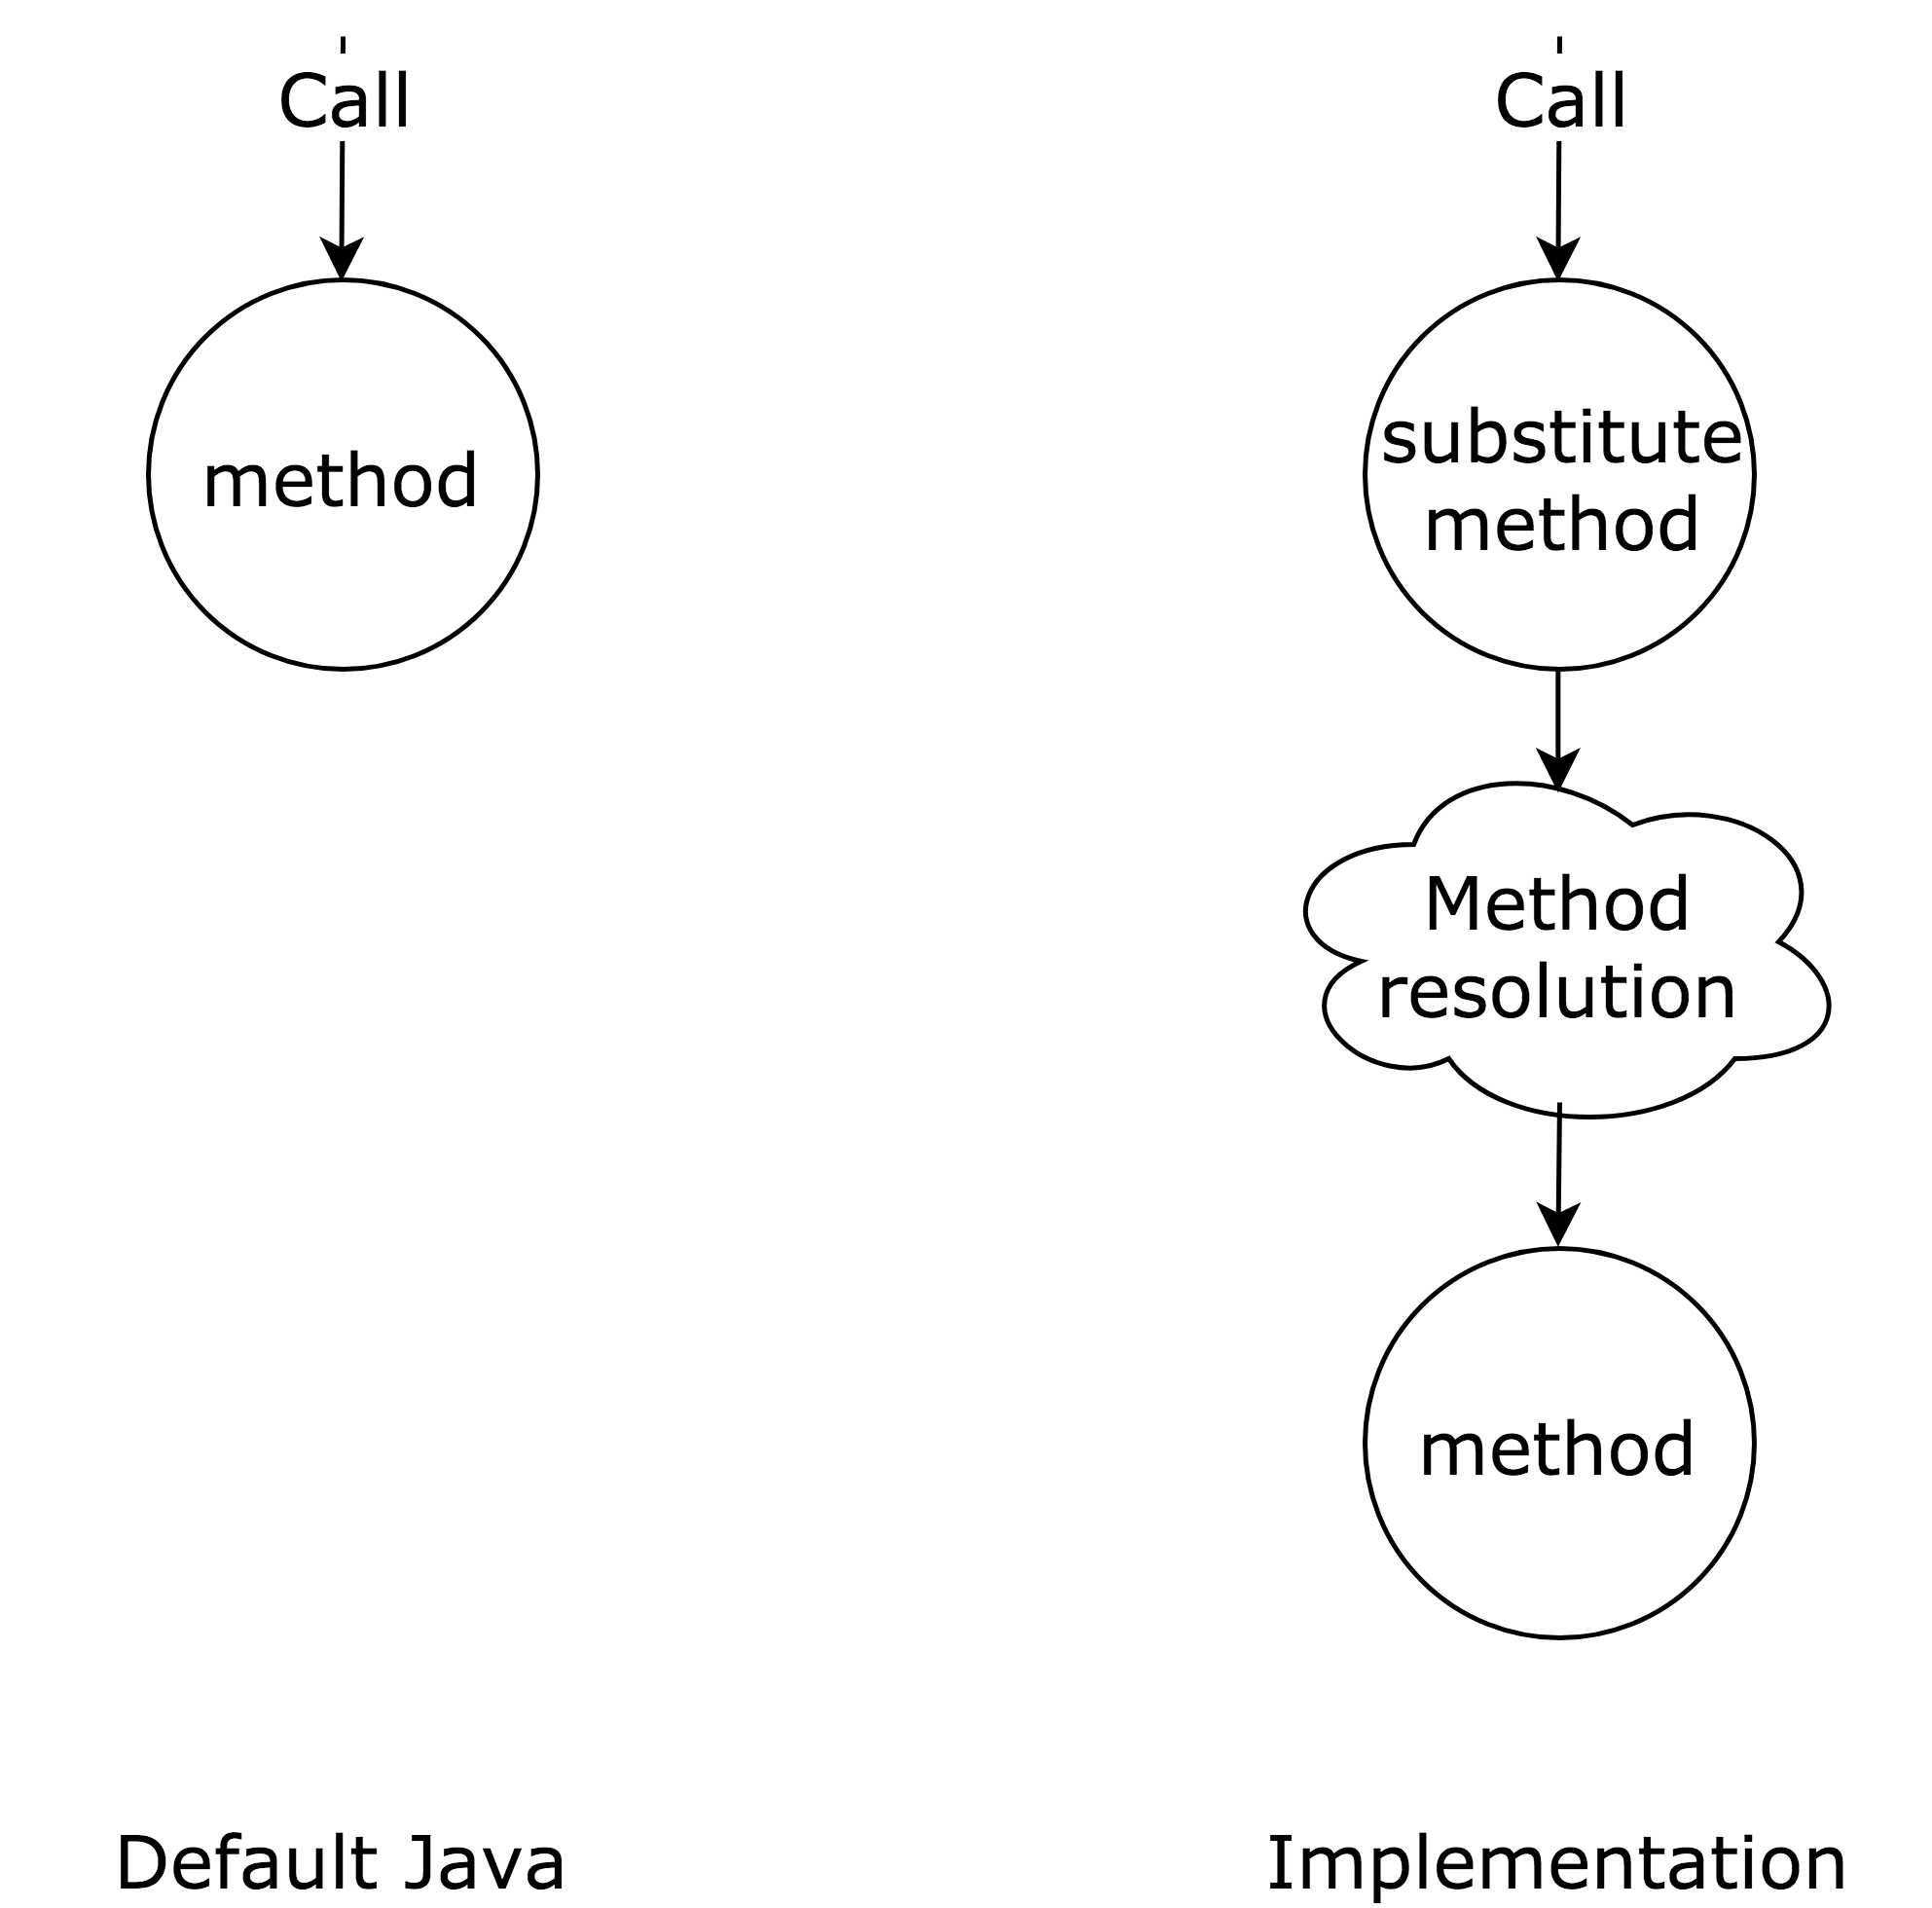
\includegraphics[height=0.78\textheight]{figures/callChain.png}
  \end{figure}
\end{frame}

\begin{frame}{Method resolution}
  \note{ 
    \begin{enumerate}
      \item When the helper class is instantiated a mapping\
        between argument types and applicable methods is generated (to create a cache)
      \item When a method is invoked: {
        \begin{enumerate}
          \item Filter methods applicable to the given arguments 
          \item Sort them by specifity
          \item Invoke the most specific
        \end{enumerate}
      }
    \end{enumerate}
  }

  \begin{enumerate}
    \item When the helper class is instantiated a mapping\
      between argument types and methods is created
    \item When a method is invoked: {
      \begin{enumerate}
        \item Filter methods applicable to the given arguments 
        \item Sort them by specifity
        \item Invoke the most specific
      \end{enumerate}
    }
  \end{enumerate}
\end{frame}

\begin{frame}{Extensions}
  \begin{itemize}
    \item Method caching
    \item Extensible to different ordering of methods
  \end{itemize}
\end{frame}

\begin{frame}{Cache Comparison}
    \begin{table}[]
      \centering
      \resizebox{\textwidth}{!}{
        \begin{tabular}{llllll}
                    & 1    & 10000 & 100000 & 1000000 &  \\
        No cache    & 154  & 156.8 & 830.8  & 7929.7  &  \\
        With cache  & 27.4 & 25.1  & 49.8   & 130.9   &  \\
        Java        & 0.2  & 0.6   & 0.7    & 0.4     & 
        \end{tabular}
      }
      \caption{Time comparison in milliseconds}
      \label{comparison-table}
      \end{table}
\end{frame}

\end{document}
